%! Author = mariuszindel
%! Date = 25.01.21

\section{Wahrscheinlichkeit}

\subsection{Wahrscheinlichkeitsrechnung}
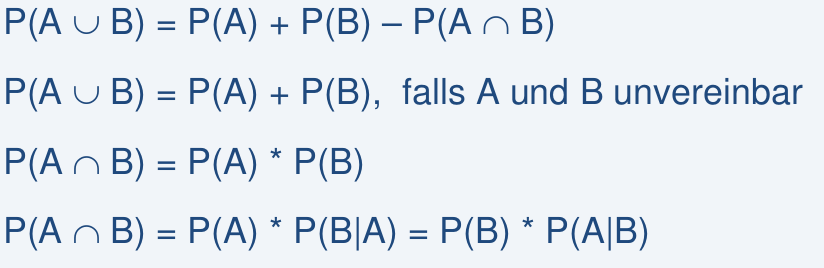
\includegraphics[width=\linewidth]{graphic/extern-reto/Wahrscheinlichkeit.png}
Lotto:\\
\colorbox{lightlightgrey}{$\frac{\binom{Gezogene}{Treffer} * \binom{Nicht-Gezogene}{Falsche}}{Anzahl aller Ergebnisse}$}\\



\subsection{Bitfehler}
\colorbox{lightlightgrey}{$P(Fehlerhaft) = 1 - P(0 Fehler)$}\\
$= 1 - $P(BitFehler)$^{Datenblock}$



\subsection{Binominalverteilung}
Wie gross ist die Wahrscheinlichkeit, dass:
\begin{itemize}
    \item genau 3
    \item weniger als 3
\end{itemize}
\colorbox{lightlightgrey}{$P(X = k) = \binom{n}{k} p^k(1 - p)^{n-k}$}\\
Wenn z.B. $\le$ 3 gesucht ist, muss für (k = 0) + (k = 1) + (k = 2) + (k = 3) gerechnet werden.

